\documentclass[]{article}
\usepackage{lmodern}
\usepackage{amssymb,amsmath}
\usepackage{ifxetex,ifluatex}
\usepackage{fixltx2e} % provides \textsubscript
\ifnum 0\ifxetex 1\fi\ifluatex 1\fi=0 % if pdftex
  \usepackage[T1]{fontenc}
  \usepackage[utf8]{inputenc}
\else % if luatex or xelatex
  \ifxetex
    \usepackage{mathspec}
  \else
    \usepackage{fontspec}
  \fi
  \defaultfontfeatures{Ligatures=TeX,Scale=MatchLowercase}
\fi
% use upquote if available, for straight quotes in verbatim environments
\IfFileExists{upquote.sty}{\usepackage{upquote}}{}
% use microtype if available
\IfFileExists{microtype.sty}{%
\usepackage{microtype}
\UseMicrotypeSet[protrusion]{basicmath} % disable protrusion for tt fonts
}{}
\usepackage[margin=1in]{geometry}
\usepackage{hyperref}
\hypersetup{unicode=true,
            pdftitle={07\_growth\_estimates\_nitrate\_compare.R},
            pdfauthor={joeybernhardt},
            pdfborder={0 0 0},
            breaklinks=true}
\urlstyle{same}  % don't use monospace font for urls
\usepackage{color}
\usepackage{fancyvrb}
\newcommand{\VerbBar}{|}
\newcommand{\VERB}{\Verb[commandchars=\\\{\}]}
\DefineVerbatimEnvironment{Highlighting}{Verbatim}{commandchars=\\\{\}}
% Add ',fontsize=\small' for more characters per line
\usepackage{framed}
\definecolor{shadecolor}{RGB}{248,248,248}
\newenvironment{Shaded}{\begin{snugshade}}{\end{snugshade}}
\newcommand{\KeywordTok}[1]{\textcolor[rgb]{0.13,0.29,0.53}{\textbf{{#1}}}}
\newcommand{\DataTypeTok}[1]{\textcolor[rgb]{0.13,0.29,0.53}{{#1}}}
\newcommand{\DecValTok}[1]{\textcolor[rgb]{0.00,0.00,0.81}{{#1}}}
\newcommand{\BaseNTok}[1]{\textcolor[rgb]{0.00,0.00,0.81}{{#1}}}
\newcommand{\FloatTok}[1]{\textcolor[rgb]{0.00,0.00,0.81}{{#1}}}
\newcommand{\ConstantTok}[1]{\textcolor[rgb]{0.00,0.00,0.00}{{#1}}}
\newcommand{\CharTok}[1]{\textcolor[rgb]{0.31,0.60,0.02}{{#1}}}
\newcommand{\SpecialCharTok}[1]{\textcolor[rgb]{0.00,0.00,0.00}{{#1}}}
\newcommand{\StringTok}[1]{\textcolor[rgb]{0.31,0.60,0.02}{{#1}}}
\newcommand{\VerbatimStringTok}[1]{\textcolor[rgb]{0.31,0.60,0.02}{{#1}}}
\newcommand{\SpecialStringTok}[1]{\textcolor[rgb]{0.31,0.60,0.02}{{#1}}}
\newcommand{\ImportTok}[1]{{#1}}
\newcommand{\CommentTok}[1]{\textcolor[rgb]{0.56,0.35,0.01}{\textit{{#1}}}}
\newcommand{\DocumentationTok}[1]{\textcolor[rgb]{0.56,0.35,0.01}{\textbf{\textit{{#1}}}}}
\newcommand{\AnnotationTok}[1]{\textcolor[rgb]{0.56,0.35,0.01}{\textbf{\textit{{#1}}}}}
\newcommand{\CommentVarTok}[1]{\textcolor[rgb]{0.56,0.35,0.01}{\textbf{\textit{{#1}}}}}
\newcommand{\OtherTok}[1]{\textcolor[rgb]{0.56,0.35,0.01}{{#1}}}
\newcommand{\FunctionTok}[1]{\textcolor[rgb]{0.00,0.00,0.00}{{#1}}}
\newcommand{\VariableTok}[1]{\textcolor[rgb]{0.00,0.00,0.00}{{#1}}}
\newcommand{\ControlFlowTok}[1]{\textcolor[rgb]{0.13,0.29,0.53}{\textbf{{#1}}}}
\newcommand{\OperatorTok}[1]{\textcolor[rgb]{0.81,0.36,0.00}{\textbf{{#1}}}}
\newcommand{\BuiltInTok}[1]{{#1}}
\newcommand{\ExtensionTok}[1]{{#1}}
\newcommand{\PreprocessorTok}[1]{\textcolor[rgb]{0.56,0.35,0.01}{\textit{{#1}}}}
\newcommand{\AttributeTok}[1]{\textcolor[rgb]{0.77,0.63,0.00}{{#1}}}
\newcommand{\RegionMarkerTok}[1]{{#1}}
\newcommand{\InformationTok}[1]{\textcolor[rgb]{0.56,0.35,0.01}{\textbf{\textit{{#1}}}}}
\newcommand{\WarningTok}[1]{\textcolor[rgb]{0.56,0.35,0.01}{\textbf{\textit{{#1}}}}}
\newcommand{\AlertTok}[1]{\textcolor[rgb]{0.94,0.16,0.16}{{#1}}}
\newcommand{\ErrorTok}[1]{\textcolor[rgb]{0.64,0.00,0.00}{\textbf{{#1}}}}
\newcommand{\NormalTok}[1]{{#1}}
\usepackage{graphicx,grffile}
\makeatletter
\def\maxwidth{\ifdim\Gin@nat@width>\linewidth\linewidth\else\Gin@nat@width\fi}
\def\maxheight{\ifdim\Gin@nat@height>\textheight\textheight\else\Gin@nat@height\fi}
\makeatother
% Scale images if necessary, so that they will not overflow the page
% margins by default, and it is still possible to overwrite the defaults
% using explicit options in \includegraphics[width, height, ...]{}
\setkeys{Gin}{width=\maxwidth,height=\maxheight,keepaspectratio}
\IfFileExists{parskip.sty}{%
\usepackage{parskip}
}{% else
\setlength{\parindent}{0pt}
\setlength{\parskip}{6pt plus 2pt minus 1pt}
}
\setlength{\emergencystretch}{3em}  % prevent overfull lines
\providecommand{\tightlist}{%
  \setlength{\itemsep}{0pt}\setlength{\parskip}{0pt}}
\setcounter{secnumdepth}{0}
% Redefines (sub)paragraphs to behave more like sections
\ifx\paragraph\undefined\else
\let\oldparagraph\paragraph
\renewcommand{\paragraph}[1]{\oldparagraph{#1}\mbox{}}
\fi
\ifx\subparagraph\undefined\else
\let\oldsubparagraph\subparagraph
\renewcommand{\subparagraph}[1]{\oldsubparagraph{#1}\mbox{}}
\fi

%%% Use protect on footnotes to avoid problems with footnotes in titles
\let\rmarkdownfootnote\footnote%
\def\footnote{\protect\rmarkdownfootnote}

%%% Change title format to be more compact
\usepackage{titling}

% Create subtitle command for use in maketitle
\newcommand{\subtitle}[1]{
  \posttitle{
    \begin{center}\large#1\end{center}
    }
}

\setlength{\droptitle}{-2em}

  \title{07\_growth\_estimates\_nitrate\_compare.R}
    \pretitle{\vspace{\droptitle}\centering\huge}
  \posttitle{\par}
    \author{joeybernhardt}
    \preauthor{\centering\large\emph}
  \postauthor{\par}
      \predate{\centering\large\emph}
  \postdate{\par}
    \date{Wed Feb 20 10:00:29 2019}


\begin{document}
\maketitle

\begin{Shaded}
\begin{Highlighting}[]
\KeywordTok{library}\NormalTok{(tidyverse)}
\end{Highlighting}
\end{Shaded}

\begin{verbatim}
## Warning: package 'tidyverse' was built under R version 3.4.2
\end{verbatim}

\begin{verbatim}
## -- Attaching packages ---------------------------------- tidyverse 1.2.1 --
\end{verbatim}

\begin{verbatim}
## √ ggplot2 3.1.0     √ purrr   0.2.5
## √ tibble  1.4.2     √ dplyr   0.7.6
## √ tidyr   0.8.1     √ stringr 1.3.1
## √ readr   1.1.1     √ forcats 0.3.0
\end{verbatim}

\begin{verbatim}
## Warning: package 'ggplot2' was built under R version 3.4.4
\end{verbatim}

\begin{verbatim}
## Warning: package 'tibble' was built under R version 3.4.3
\end{verbatim}

\begin{verbatim}
## Warning: package 'tidyr' was built under R version 3.4.4
\end{verbatim}

\begin{verbatim}
## Warning: package 'purrr' was built under R version 3.4.4
\end{verbatim}

\begin{verbatim}
## Warning: package 'dplyr' was built under R version 3.4.4
\end{verbatim}

\begin{verbatim}
## Warning: package 'stringr' was built under R version 3.4.4
\end{verbatim}

\begin{verbatim}
## Warning: package 'forcats' was built under R version 3.4.3
\end{verbatim}

\begin{verbatim}
## -- Conflicts ------------------------------------- tidyverse_conflicts() --
## x dplyr::filter() masks stats::filter()
## x dplyr::lag()    masks stats::lag()
\end{verbatim}

\begin{Shaded}
\begin{Highlighting}[]
\KeywordTok{library}\NormalTok{(cowplot)}
\end{Highlighting}
\end{Shaded}

\begin{verbatim}
## Warning: package 'cowplot' was built under R version 3.4.4
\end{verbatim}

\begin{verbatim}
## 
## Attaching package: 'cowplot'
\end{verbatim}

\begin{verbatim}
## The following object is masked from 'package:ggplot2':
## 
##     ggsave
\end{verbatim}

\begin{Shaded}
\begin{Highlighting}[]
\KeywordTok{library}\NormalTok{(broom)}
\KeywordTok{library}\NormalTok{(readxl)}
\end{Highlighting}
\end{Shaded}

\begin{verbatim}
## Warning: package 'readxl' was built under R version 3.4.4
\end{verbatim}

\begin{Shaded}
\begin{Highlighting}[]
\KeywordTok{library}\NormalTok{(janitor)}
\end{Highlighting}
\end{Shaded}

\begin{verbatim}
## Warning: package 'janitor' was built under R version 3.4.4
\end{verbatim}

\begin{Shaded}
\begin{Highlighting}[]
\KeywordTok{library}\NormalTok{(plotrix)}
\end{Highlighting}
\end{Shaded}

\begin{verbatim}
## Warning: package 'plotrix' was built under R version 3.4.4
\end{verbatim}

\begin{Shaded}
\begin{Highlighting}[]
\KeywordTok{library}\NormalTok{(here)}
\end{Highlighting}
\end{Shaded}

\begin{verbatim}
## here() starts at /Users/joeybernhardt/Documents/Narwani/ChlamEE-R-star
\end{verbatim}

\begin{Shaded}
\begin{Highlighting}[]
\NormalTok{treatments <-}\StringTok{ }\KeywordTok{read_excel}\NormalTok{(}\KeywordTok{here}\NormalTok{(}\StringTok{"data-general"}\NormalTok{, }\StringTok{"ChlamEE_Treatments_JB.xlsx"}\NormalTok{)) %>%}\StringTok{ }
\StringTok{    }\KeywordTok{clean_names}\NormalTok{() %>%}\StringTok{ }
\StringTok{    }\KeywordTok{mutate}\NormalTok{(}\DataTypeTok{treatment =} \KeywordTok{ifelse}\NormalTok{(}\KeywordTok{is.na}\NormalTok{(treatment), }\StringTok{"none"}\NormalTok{, treatment)) %>%}\StringTok{ }
\StringTok{    }\KeywordTok{filter}\NormalTok{(population !=}\StringTok{ "cc1629"}\NormalTok{) }
\end{Highlighting}
\end{Shaded}

\begin{verbatim}
## Warning: package 'bindrcpp' was built under R version 3.4.4
\end{verbatim}

\begin{Shaded}
\begin{Highlighting}[]
\CommentTok{# compare growth rate estimates -------------------------------------------}

\NormalTok{logistic <-}\StringTok{ }\KeywordTok{read_csv}\NormalTok{(}\KeywordTok{here}\NormalTok{(}\StringTok{"data-processed"}\NormalTok{, }\StringTok{"nitrate_exp_growth_logistic.csv"}\NormalTok{)) %>%}\StringTok{ }
\StringTok{    }\KeywordTok{select}\NormalTok{(population, ancestor_id, treatment, nitrate_concentration, estimate) %>%}\StringTok{ }
\StringTok{    }\KeywordTok{mutate}\NormalTok{(}\DataTypeTok{method  =} \StringTok{"logistic"}\NormalTok{) %>%}\StringTok{ }
\StringTok{    }\KeywordTok{distinct}\NormalTok{(population, ancestor_id, treatment, nitrate_concentration, estimate) %>%}\StringTok{ }
\StringTok{    }\KeywordTok{filter}\NormalTok{(!}\KeywordTok{is.na}\NormalTok{(ancestor_id)) %>%}\StringTok{ }
\StringTok{    }\KeywordTok{mutate}\NormalTok{(}\DataTypeTok{population =} \KeywordTok{as.character}\NormalTok{(population)) %>%}\StringTok{ }
\StringTok{    }\KeywordTok{mutate}\NormalTok{(}\DataTypeTok{method =} \StringTok{"intrinsic rate of incr via logistic"}\NormalTok{)}
\end{Highlighting}
\end{Shaded}

\begin{verbatim}
## Parsed with column specification:
## cols(
##   .default = col_character(),
##   population = col_integer(),
##   estimate = col_double(),
##   std.error = col_double(),
##   statistic = col_double(),
##   p.value = col_double(),
##   conf.low = col_double(),
##   conf.high = col_double(),
##   nitrate_concentration = col_double(),
##   plate_key = col_integer(),
##   nitrate_level = col_integer(),
##   plate = col_integer(),
##   multitron = col_integer(),
##   slot = col_integer()
## )
\end{verbatim}

\begin{verbatim}
## See spec(...) for full column specifications.
\end{verbatim}

\begin{verbatim}
## Warning in rbind(names(probs), probs_f): number of columns of result is not
## a multiple of vector length (arg 1)
\end{verbatim}

\begin{verbatim}
## Warning: 200 parsing failures.
## row # A tibble: 5 x 5 col     row col      expected  actual file                                     expected   <int> <chr>    <chr>     <chr>  <chr>                                    actual 1  1281 populat~ an integ~ anc2   '/Users/joeybernhardt/Documents/Narwani~ file 2  1282 populat~ an integ~ anc2   '/Users/joeybernhardt/Documents/Narwani~ row 3  1283 populat~ an integ~ anc2   '/Users/joeybernhardt/Documents/Narwani~ col 4  1284 populat~ an integ~ anc2   '/Users/joeybernhardt/Documents/Narwani~ expected 5  1285 populat~ an integ~ anc2   '/Users/joeybernhardt/Documents/Narwani~
## ... ................. ... .......................................................................... ........ .......................................................................... ...... .......................................................................... .... .......................................................................... ... .......................................................................... ... .......................................................................... ........ ..........................................................................
## See problems(...) for more details.
\end{verbatim}

\begin{Shaded}
\begin{Highlighting}[]
\NormalTok{eyeball <-}\StringTok{ }\KeywordTok{read_csv}\NormalTok{(}\KeywordTok{here}\NormalTok{(}\StringTok{"data-processed"}\NormalTok{, }\StringTok{"nitrate_exp_growth_eyeball.csv"}\NormalTok{)) %>%}\StringTok{ }
\StringTok{    }\KeywordTok{select}\NormalTok{(population, ancestor_id, treatment, nitrate_concentration.x, estimate) %>%}
\StringTok{    }\KeywordTok{rename}\NormalTok{(}\DataTypeTok{nitrate_concentration =} \NormalTok{nitrate_concentration.x) %>%}\StringTok{ }
\StringTok{    }\KeywordTok{distinct}\NormalTok{(population, ancestor_id, treatment, nitrate_concentration, estimate) %>%}\StringTok{ }
\StringTok{    }\KeywordTok{filter}\NormalTok{(!}\KeywordTok{is.na}\NormalTok{(population))%>%}\StringTok{ }
\StringTok{    }\KeywordTok{mutate}\NormalTok{(}\DataTypeTok{population =} \KeywordTok{as.character}\NormalTok{(population)) %>%}\StringTok{ }
\StringTok{    }\KeywordTok{mutate}\NormalTok{(}\DataTypeTok{method  =} \StringTok{"eyeball-exponential"}\NormalTok{)}
\end{Highlighting}
\end{Shaded}

\begin{verbatim}
## Parsed with column specification:
## cols(
##   .default = col_character(),
##   nitrate_concentration.x = col_integer(),
##   population = col_integer(),
##   estimate = col_double(),
##   std.error = col_double(),
##   statistic = col_double(),
##   p.value = col_double(),
##   plate_key = col_integer(),
##   nitrate_level = col_integer(),
##   plate = col_integer(),
##   multitron = col_integer(),
##   slot = col_integer(),
##   nitrate_concentration.y = col_double()
## )
## See spec(...) for full column specifications.
\end{verbatim}

\begin{verbatim}
## Warning in rbind(names(probs), probs_f): number of columns of result is not
## a multiple of vector length (arg 1)
\end{verbatim}

\begin{verbatim}
## Warning: 8000 parsing failures.
## row # A tibble: 5 x 5 col     row col      expected  actual file                                     expected   <int> <chr>    <chr>     <chr>  <chr>                                    actual 1  5121 populat~ an integ~ anc2   '/Users/joeybernhardt/Documents/Narwani~ file 2  5122 populat~ an integ~ anc2   '/Users/joeybernhardt/Documents/Narwani~ row 3  5123 populat~ an integ~ anc2   '/Users/joeybernhardt/Documents/Narwani~ col 4  5124 populat~ an integ~ anc2   '/Users/joeybernhardt/Documents/Narwani~ expected 5  5125 populat~ an integ~ anc2   '/Users/joeybernhardt/Documents/Narwani~
## ... ................. ... .......................................................................... ........ .......................................................................... ...... .......................................................................... .... .......................................................................... ... .......................................................................... ... .......................................................................... ........ ..........................................................................
## See problems(...) for more details.
\end{verbatim}

\begin{Shaded}
\begin{Highlighting}[]
\NormalTok{AIC_exp <-}\StringTok{ }\KeywordTok{read_csv}\NormalTok{(}\KeywordTok{here}\NormalTok{(}\StringTok{"data-processed"}\NormalTok{, }\StringTok{"nitrate_exp_growth_w_growthtools_AIC.csv"}\NormalTok{)) %>%}\StringTok{ }
\StringTok{    }\KeywordTok{rename}\NormalTok{(}\DataTypeTok{estimate =} \NormalTok{mu) %>%}\StringTok{ }
\StringTok{    }\KeywordTok{mutate}\NormalTok{(}\DataTypeTok{method =} \StringTok{"exponential via pw regression and AIC"}\NormalTok{) %>%}\StringTok{ }
\StringTok{    }\KeywordTok{mutate}\NormalTok{(}\DataTypeTok{population =} \KeywordTok{as.character}\NormalTok{(population))}
\end{Highlighting}
\end{Shaded}

\begin{verbatim}
## Parsed with column specification:
## cols(
##   well_plate = col_character(),
##   mu = col_double(),
##   best.model = col_character(),
##   best.se = col_double(),
##   population = col_character(),
##   nitrate_concentration = col_integer()
## )
\end{verbatim}

\begin{Shaded}
\begin{Highlighting}[]
\NormalTok{AIC_exp <-}\StringTok{ }\KeywordTok{left_join}\NormalTok{(AIC_exp, treatments)}
\end{Highlighting}
\end{Shaded}

\begin{verbatim}
## Joining, by = "population"
\end{verbatim}

\begin{Shaded}
\begin{Highlighting}[]
\NormalTok{AICc_exp <-}\StringTok{ }\KeywordTok{read_csv}\NormalTok{(}\KeywordTok{here}\NormalTok{(}\StringTok{"data-processed"}\NormalTok{, }\StringTok{"nitrate_exp_growth_w_growthtools.csv"}\NormalTok{)) %>%}\StringTok{ }
\StringTok{    }\KeywordTok{rename}\NormalTok{(}\DataTypeTok{estimate =} \NormalTok{mu) %>%}\StringTok{ }
\StringTok{    }\KeywordTok{mutate}\NormalTok{(}\DataTypeTok{method =} \StringTok{"exponential via pw regression and AICc"}\NormalTok{) %>%}\StringTok{ }
\StringTok{    }\KeywordTok{mutate}\NormalTok{(}\DataTypeTok{population =} \KeywordTok{as.character}\NormalTok{(population))}
\end{Highlighting}
\end{Shaded}

\begin{verbatim}
## Parsed with column specification:
## cols(
##   well_plate = col_character(),
##   mu = col_double(),
##   best.model = col_character(),
##   best.se = col_double(),
##   population = col_character(),
##   nitrate_concentration = col_integer()
## )
\end{verbatim}

\begin{Shaded}
\begin{Highlighting}[]
\NormalTok{AICc_exp <-}\StringTok{ }\KeywordTok{left_join}\NormalTok{(AICc_exp, treatments)}
\end{Highlighting}
\end{Shaded}

\begin{verbatim}
## Joining, by = "population"
\end{verbatim}

\begin{Shaded}
\begin{Highlighting}[]
\NormalTok{all_growth_estimates <-}\StringTok{ }\KeywordTok{bind_rows}\NormalTok{(logistic, eyeball, AIC_exp, AICc_exp)}


\NormalTok{all_growth_estimates %>%}
\StringTok{    }\KeywordTok{group_by}\NormalTok{(population, nitrate_concentration) %>%}\StringTok{ }
\StringTok{    }\KeywordTok{ggplot}\NormalTok{(}\KeywordTok{aes}\NormalTok{(}\DataTypeTok{x =} \NormalTok{nitrate_concentration, }\DataTypeTok{y =} \NormalTok{estimate, }\DataTypeTok{color =} \NormalTok{method)) +}\StringTok{ }\KeywordTok{geom_point}\NormalTok{(}\DataTypeTok{shape =} \DecValTok{1}\NormalTok{) +}
\StringTok{    }\KeywordTok{facet_grid}\NormalTok{(ancestor_id ~}\StringTok{ }\NormalTok{treatment)}
\end{Highlighting}
\end{Shaded}

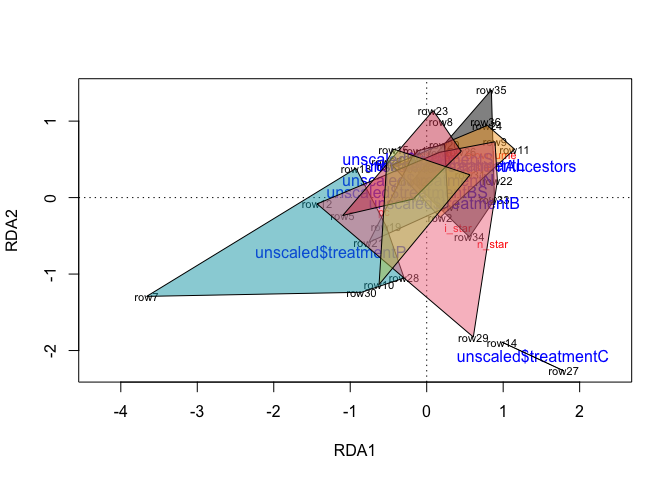
\includegraphics{07_growth_estimates_nitrate_compare_files/figure-latex/unnamed-chunk-1-1.pdf}

\begin{Shaded}
\begin{Highlighting}[]
\KeywordTok{ggsave}\NormalTok{(}\KeywordTok{here}\NormalTok{(}\StringTok{"figures"}\NormalTok{, }\StringTok{"comparison_nitrate_monod.png"}\NormalTok{), }\DataTypeTok{width =} \DecValTok{15}\NormalTok{, }\DataTypeTok{height =} \DecValTok{6}\NormalTok{)}


\NormalTok{all_growth_estimates %>%}\StringTok{ }
\StringTok{    }\KeywordTok{group_by}\NormalTok{(population, nitrate_concentration, ancestor_id, treatment, method) %>%}\StringTok{ }
\StringTok{    }\KeywordTok{summarise_each}\NormalTok{(}\KeywordTok{funs}\NormalTok{(mean, std.error), estimate) %>%}\StringTok{ }
\StringTok{    }\KeywordTok{ggplot}\NormalTok{(}\KeywordTok{aes}\NormalTok{(}\DataTypeTok{x =} \NormalTok{nitrate_concentration, }\DataTypeTok{y =} \NormalTok{mean, }\DataTypeTok{color =} \NormalTok{method)) +}\StringTok{ }\KeywordTok{geom_point}\NormalTok{(}\DataTypeTok{shape=}\DecValTok{1}\NormalTok{) +}
\StringTok{    }\KeywordTok{geom_errorbar}\NormalTok{(}\KeywordTok{aes}\NormalTok{(}\DataTypeTok{ymin =} \NormalTok{mean -}\StringTok{ }\NormalTok{std.error, }\DataTypeTok{ymax =} \NormalTok{mean +}\StringTok{ }\NormalTok{std.error), }\DataTypeTok{width =} \FloatTok{0.1}\NormalTok{) +}
\StringTok{    }\KeywordTok{facet_grid}\NormalTok{(ancestor_id ~}\StringTok{ }\NormalTok{treatment) +}\StringTok{ }\KeywordTok{ylab}\NormalTok{(}\StringTok{"Mean growth rate (/day)"}\NormalTok{) +}\StringTok{ }\KeywordTok{xlab}\NormalTok{(}\StringTok{"Nitrate (uM)"}\NormalTok{)}
\end{Highlighting}
\end{Shaded}

\begin{verbatim}
## `summarise_each()` is deprecated.
## Use `summarise_all()`, `summarise_at()` or `summarise_if()` instead.
## To map `funs` over a selection of variables, use `summarise_at()`
\end{verbatim}

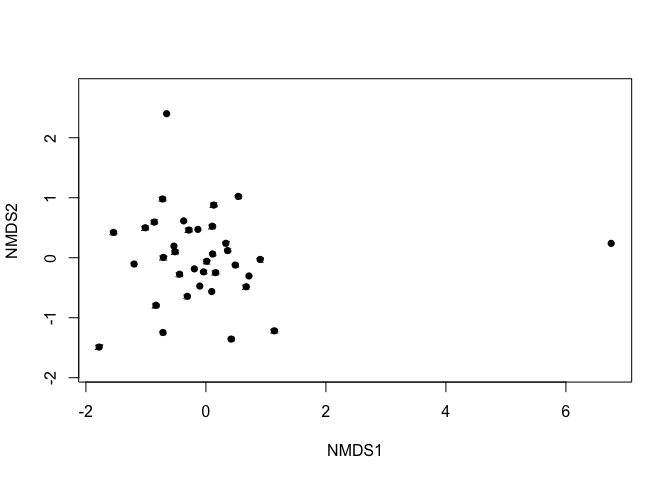
\includegraphics{07_growth_estimates_nitrate_compare_files/figure-latex/unnamed-chunk-1-2.pdf}

\begin{Shaded}
\begin{Highlighting}[]
\KeywordTok{ggsave}\NormalTok{(}\KeywordTok{here}\NormalTok{(}\StringTok{"figures"}\NormalTok{, }\StringTok{"comparison_nitrate_monod_means.png"}\NormalTok{), }\DataTypeTok{width =} \DecValTok{17}\NormalTok{, }\DataTypeTok{height =} \DecValTok{6}\NormalTok{)}
\end{Highlighting}
\end{Shaded}


\end{document}
